%==========================================================
% AGENTIC DOCUMENT PROCESSOR — BEAMER PRESENTATION
% Upload to Overleaf (pdflatex) — compile twice for refs
%==========================================================
\documentclass[aspectratio=169,t]{beamer}

\usetheme{Madrid}
\usecolortheme{whale}
\setbeamertemplate{navigation symbols}{}
\setbeamertemplate{footline}[frame number]
\setbeamerfont{frametitle}{size=\normalsize,series=\bfseries}

%-------- Packages --------
\usepackage[utf8]{inputenc}
\usepackage[T1]{fontenc}
\usepackage{lmodern}
\usepackage{booktabs}
\usepackage{colortbl}
\usepackage{xcolor}
\usepackage{tikz}
\usepackage{pgfplots}
\pgfplotsset{compat=1.18}
\usepackage{fontawesome5}
\usepackage{tcolorbox}
\tcbuselibrary{skins}
\usepackage{array}
\usepackage{newunicodechar}
\newunicodechar{→}{\ensuremath{\rightarrow}}
\newunicodechar{—}{---}
\usetikzlibrary{shapes.geometric,arrows.meta,positioning,
                shadows,backgrounds}

%-------- Colors --------
\definecolor{primary}{RGB}{25,85,160}
\definecolor{secondary}{RGB}{0,140,200}
\definecolor{accent}{RGB}{230,120,0}
\definecolor{success}{RGB}{46,160,67}
\definecolor{danger}{RGB}{200,50,50}
\definecolor{lgray}{RGB}{245,246,250}
\definecolor{groqcol}{RGB}{110,45,170}
\definecolor{brcol}{RGB}{30,120,60}

\setbeamercolor{palette primary}{bg=primary}
\setbeamercolor{palette secondary}{bg=secondary}
\setbeamercolor{palette quaternary}{bg=primary}
\setbeamercolor{block title}{bg=primary,fg=white}
\setbeamercolor{alerted text}{fg=accent}

%-------- tcolorbox helpers --------
\tcbset{
  cblock/.style={enhanced,colback=lgray,colframe=primary!60,
    sharp corners,boxrule=0.5pt,left=4pt,right=4pt,
    top=2pt,bottom=2pt,fontupper=\ttfamily\scriptsize},
  hibox/.style={enhanced,colback=#1!8,colframe=#1,
    sharp corners,boxrule=0.8pt,left=5pt,right=5pt,
    top=3pt,bottom=3pt},
  titled/.style={enhanced,colback=lgray,colframe=primary,
    fonttitle=\bfseries\small,coltitle=white,
    attach boxed title to top left,
    boxed title style={colback=primary,sharp corners},
    sharp corners,boxrule=0.5pt,
    left=5pt,right=5pt,top=8pt,bottom=4pt}
}

%-------- Meta --------
\title[Agentic Doc Processor]{\textbf{Agentic Document Processor}}
\subtitle{Classify · Extract · Validate · Redact · Report}
\author{\textbf{[Your Name]}}
\institute{Agentic AI Systems --- Capstone Project}
\date{February 2026}

%==========================================================
\begin{document}
%==========================================================

%------ TITLE ------
\begin{frame}[plain]
\begin{tikzpicture}[remember picture,overlay]
  \fill[primary](current page.north west)
    rectangle([yshift=-2cm]current page.north east);
  \fill[accent]([yshift=-2cm]current page.north west)
    rectangle([yshift=-2.15cm]current page.north east);
  \fill[primary!80](current page.south west)
    rectangle([yshift=0.6cm]current page.south east);
\end{tikzpicture}
\vspace{0.5cm}
\begin{center}
  {\color{white}\fontsize{24}{29}\selectfont\bfseries
    Agentic Document Processor}\\[6pt]
  {\color{white!80}\large
    LangGraph · Groq · Amazon Bedrock · Presidio}\\[10pt]
  {\color{accent}\rule{9cm}{1.4pt}}\\[8pt]
  {\color{white}\small
    Classify \;·\; Extract \;·\; Validate \;·\; Redact \;·\; Report}
\end{center}
\vspace{0.55cm}
\begin{center}
  
\begin{tikzpicture}
    \node[fill=white,rounded corners=5pt,inner sep=7pt,
          draw=accent,line width=1pt]{%
      \footnotesize\color{primary}
      \faProjectDiagram~Multi-Agent \quad
      \faRobot~LangGraph \quad
      \faUserSecret~PII Redaction \quad
      \faChartBar~Responsible AI};
  \end{tikzpicture}
\end{center}
\end{frame}

%------ AGENDA ------
\begin{frame}{Agenda}
\begin{columns}[T]
\column{0.48\textwidth}
\begin{tcolorbox}[titled,title={\faList~Topics}]
\begin{enumerate}\setlength\itemsep{5pt}\small
  \item[\textcolor{accent}{\bfseries 1}]
    Problem Statement
  \item[\textcolor{accent}{\bfseries 2}]
    Solution --- What \& Why
  \item[\textcolor{accent}{\bfseries 3}]
    High-Level Architecture
  \item[\textcolor{accent}{\bfseries 4}]
    Deep Dive: Codebase
\end{enumerate}
\end{tcolorbox}
\column{0.48\textwidth}
\begin{tcolorbox}[titled,title={\faChartLine~Outcomes}]
\begin{enumerate}\setlength\itemsep{5pt}\small
  \item[\textcolor{accent}{\bfseries 5}]
    Evaluation \& Performance
  \item[\textcolor{accent}{\bfseries 6}]
    Salient Features
  \item[\textcolor{accent}{\bfseries 7}]
    Live Demo
  \item[\textcolor{accent}{\bfseries 8}]
    Future Scope
\end{enumerate}
\end{tcolorbox}
\end{columns}
\end{frame}

%==========================================================
\section{Problem Statement}
%==========================================================

\begin{frame}{Problem Statement}
\begin{tcolorbox}[hibox=danger,
  title={\faExclamationTriangle~The Problem},
  fonttitle=\bfseries\small,coltitle=white,
  attach boxed title to top left,
  boxed title style={colback=danger,sharp corners}]
\small
Organizations process thousands of heterogeneous documents daily ---
invoices, resumes, medical records, IDs, transcripts ---
requiring \textbf{manual classification, field extraction, and PII handling}.
This is error-prone, slow, and non-auditable.
\end{tcolorbox}

\vspace{8pt}
\begin{columns}[T]
\column{0.32\textwidth}
\begin{tcolorbox}[hibox=danger]
\centering\textbf{\faClock~Manual \& Slow}\\[4pt]
\scriptsize Reviewers handle 10--50 docs/day.
Complex multi-format documents require different tools per format.
\end{tcolorbox}
\column{0.32\textwidth}
\begin{tcolorbox}[hibox=danger]
\centering\textbf{\faLock~PII Exposure}\\[4pt]
\scriptsize SSN, Aadhaar, emails, DOBs leak unmasked into downstream
analytics without systematic redaction.
\end{tcolorbox}
\column{0.32\textwidth}
\begin{tcolorbox}[hibox=danger]
\centering\textbf{\faEye~No Audit Trail}\\[4pt]
\scriptsize GDPR / HIPAA require decision traces ---
manual processing leaves no structured log of
who/what acted on each document.
\end{tcolorbox}
\end{columns}

\vspace{8pt}
\begin{columns}[T]
\column{0.6\textwidth}
\textbf{Document Types in Scope:}\quad
\scriptsize
\faReceipt~Financial \;
\faUser~Resume \;
\faBriefcase~Job Offer \;
\faNotesMedical~Medical \;
\faIdCard~Identity \;
\faGraduationCap~Academic

\column{0.38\textwidth}
\textbf{Regulatory Drivers:}\quad
\scriptsize GDPR · HIPAA · India DPDP Act 2023
\end{columns}
\end{frame}

%==========================================================
\section{Solution}
%==========================================================

\begin{frame}{Solution --- What \& Why}
\begin{tcolorbox}[hibox=success,
  title={\faRocket~What We Built},
  fonttitle=\bfseries\small,coltitle=white,
  attach boxed title to top left,
  boxed title style={colback=success,sharp corners}]
\small
A \textbf{local, agentic pipeline} that ingests any document, routes it through
\textbf{6 specialised AI agents} orchestrated by LangGraph, and produces
\textbf{validated JSON + redacted text + Responsible AI audit log}.
\end{tcolorbox}

\vspace{8pt}
\begin{columns}[T]
\column{0.48\textwidth}
\begin{tcolorbox}[titled,title={\faQuestion~Why LangGraph?}]
\begin{itemize}\small\setlength\itemsep{4pt}
  \item \textbf{Shared state} --- one \texttt{DocumentState}
        TypedDict flows through every node
  \item \textbf{Conditional routing} --- self-repair fires
        only when accuracy $<$ 80\%
  \item \textbf{MemorySaver} --- checkpoints state after
        every node; survives crashes
  \item \textbf{Graph visualisation} --- auto-generates
        Mermaid diagram of the pipeline
\end{itemize}
\end{tcolorbox}

\column{0.48\textwidth}
\begin{tcolorbox}[titled,title={\faQuestion~Why Groq + Bedrock?}]
\begin{itemize}\small\setlength\itemsep{4pt}
  \item \textbf{Groq} (primary) --- llama-3.1-8b-instant,
        300+ tokens/sec, $\sim$1.5 s end-to-end
  \item \textbf{Bedrock Claude 3.5 Haiku} (fallback) ---
        AWS SLA, $\sim$3--8 s
  \item \textbf{HuggingFace API} --- tertiary fallback
  \item \textbf{Local phi-2} --- offline last resort,
        zero API dependency
\end{itemize}
\end{tcolorbox}
\end{columns}
\end{frame}

%==========================================================
\section{Architecture}
%==========================================================

\begin{frame}{High-Level Architecture}
\centering
\resizebox{0.97\textwidth}{!}{%
\begin{tikzpicture}[
  node distance=0.9cm and 1.1cm,
  ag/.style={rectangle,rounded corners=7pt,
    minimum width=2.1cm,minimum height=0.85cm,
    draw=primary,fill=secondary!12,
    font=\small\bfseries,text centered,text width=2.1cm,
    drop shadow},
  io/.style={rectangle,rounded corners=4pt,
    minimum width=1.9cm,minimum height=0.75cm,
    draw=darkgray!60,fill=lgray,
    font=\scriptsize,text centered,text width=1.9cm},
  dc/.style={diamond,minimum width=1.8cm,minimum height=0.9cm,
    draw=accent,fill=accent!12,
    font=\scriptsize\bfseries,text centered,aspect=2},
  llm/.style={rectangle,rounded corners=3pt,
    minimum width=1.9cm,minimum height=0.6cm,
    font=\scriptsize,text centered,text width=1.9cm},
  fl/.style={->,>=Stealth,thick,draw=primary!70},
  bk/.style={->,>=Stealth,thick,dashed,draw=accent},
  lf/.style={->,>=Stealth,thin,dashed,draw=groqcol!50}
]
% ---- main row ----
\node[io](inp){\faFileAlt\\\textbf{Input Doc}\\\tiny PDF/TXT/IMG};
\node[ag,right=of inp](ldr){\faDownload\\Document\\Loader};
\node[ag,right=of ldr](cls){\faTags\\Classifier\\Agent};
\node[ag,right=of cls](ext){\faCogs\\Extractor\\Agent};
\node[ag,right=of ext](val){\faCheckDouble\\Validator\\Agent};
\node[dc,right=of val](dec){Valid?};
\node[ag,right=of dec](red){\faUserSecret\\Redactor\\Agent};
\node[ag,right=of red](rep){\faChartBar\\Reporter\\Agent};
\node[io,right=of rep](out){\faFileCode\\\textbf{Output}\\\tiny JSON + CSV};

% ---- self-repair ----
\node[ag,below=1cm of dec](rpn){\faWrench\\Self-Repair\\Node};

% ---- LLM row ----
\node[llm,below=2cm of cls,fill=groqcol!12,draw=groqcol]
  (g1){\textcolor{groqcol}{\textbf{Groq}}\\\scriptsize Primary};
\node[llm,right=0.2cm of g1,fill=brcol!12,draw=brcol]
  (g2){\textcolor{brcol}{\textbf{Bedrock}}\\\scriptsize Fallback};
\node[llm,right=0.2cm of g2,fill=secondary!12,draw=secondary]
  (g3){HuggingFace\\\scriptsize Tertiary};
\node[llm,right=0.2cm of g3,fill=lgray,draw=darkgray!60]
  (g4){Local phi-2\\\scriptsize Last resort};

% ---- flows ----
\draw[fl](inp)--(ldr);
\draw[fl](ldr)--(cls);
\draw[fl](cls)--(ext);
\draw[fl](ext)--(val);
\draw[fl](val)--(dec);
\draw[fl](dec)--node[above,font=\tiny,text=success]{\faCheck~Yes}(red);
\draw[fl](red)--(rep);
\draw[fl](rep)--(out);
\draw[bk](dec)--node[right,font=\tiny,text=danger]{\faTimes~No}(rpn);
\draw[bk](rpn.west)--+(-0.35,0)|-
  node[font=\tiny,left,text=accent,pos=0.7]{retry}(val.south);

% ---- LLM taps ----
\draw[lf](g1.north)--++(0,0.3)-|(cls.south);
\draw[lf](g1.north)--++(0,0.3)-|(ext.south);
\draw[lf](g1.north)--++(0,0.3)-|(val.south);
\draw[lf](g1.north)--++(0,0.3)-|(rpn.south);
\draw[lf](g1.north)--++(0,0.3)-|(red.south);
\draw[lf,draw=accent!50](g1)--(g2)
  node[above,font=\tiny,pos=0.5]{fallback};
\draw[lf,draw=accent!50](g2)--(g3)
  node[above,font=\tiny,pos=0.5]{fallback};
\draw[lf,draw=accent!50](g3)--(g4)
  node[above,font=\tiny,pos=0.5]{fallback};
\end{tikzpicture}
}
\end{frame}

%==========================================================
\section{Deep Dive}
%==========================================================

\begin{frame}{Deep Dive --- Document Ingestion \& Classification}
\begin{columns}[T]
\column{0.48\textwidth}
\textbf{\faDownload~\texttt{utils/document\_loader.py}}\\[4pt]
Single entry point. Detects format, picks correct loader, returns \texttt{raw\_text: str} into \texttt{DocumentState}.

\vspace{6pt}
\begin{tabular}{@{}lll@{}}
\toprule
\rowcolor{primary!10}\textbf{Format} & \textbf{Loader} \\
\midrule
PDF (digital)   & PyPDFLoader \\
TXT / MD        & TextLoader \\
DOCX            & UnstructuredWord \\
PNG / JPG / TIFF & Tesseract OCR \\
Scanned PDF     & pdf2image + Tesseract \\
\bottomrule
\end{tabular}

\vspace{5pt}
\begin{tcolorbox}[hibox=accent]
\scriptsize
\textbf{Scanned PDF fallback:} if \texttt{PyPDF2} returns $<$50 chars/page,
converts the page to a PIL image and re-runs Tesseract.
Handles mixed digital + scanned PDFs transparently.
\end{tcolorbox}

\column{0.48\textwidth}
\textbf{\faTags~\texttt{agents/classifier\_agent.py}}\\[4pt]
Classifies into one of 6 \texttt{DocumentType} values using an
LLM with a \textbf{first-match decision-tree prompt}.

\vspace{6pt}
\begin{tcolorbox}[cblock]
PROMPT (decision tree, 600-char window):\\
1. Payment/billing? → financial\_document\\
2. Work Experience / Skills? → resume\\
3. Formal offer letter? → job\_offer\\
4. Medical diagnosis? → medical\_record\\
5. Photo ID / passport? → id\_document\\
6. Institution grades/degree? → academic\\[4pt]
Returns: \{doc\_type, confidence, reasoning\}
\end{tcolorbox}

\vspace{5pt}
\begin{itemize}\scriptsize\setlength\itemsep{2pt}
  \item 60+ alias mappings (``CV'', ``mark sheet'', ``appointment letter'')
  \item 3-strategy JSON parser: direct \textrightarrow{} strip fences
        \textrightarrow{} brace-count
  \item Falls back to \texttt{UNKNOWN} --- never crashes
\end{itemize}
\end{columns}
\end{frame}

\begin{frame}{Deep Dive --- Extraction \& Validation}
\begin{columns}[T]
\column{0.48\textwidth}
\textbf{\faCogs~\texttt{agents/extractor\_agent.py}}\\[4pt]
Maps \texttt{doc\_type} to a Pydantic schema, sends schema +
few-shot example to LLM, returns structured JSON fields.

\vspace{5pt}
\begin{tabular}{@{}ll@{}}
\toprule
\rowcolor{primary!10}\textbf{Schema} & \textbf{Fields} \\
\midrule
ResumeFields & 11 (incl.\ nested lists) \\
JobOfferFields & 13 \\
FinancialDocumentFields & 12 \\
MedicalRecordFields & 11 \\
IdDocumentFields & 11 \\
AcademicFields & 10 \\
\bottomrule
\end{tabular}

\vspace{5pt}
\begin{itemize}\scriptsize\setlength\itemsep{2pt}
  \item Texts $>$3000 chars chunked with 200-char overlap
  \item Chunks merged --- non-null values never overwritten
  \item Dates normalised to ISO\,8601; amounts to float
  \item All fields optional --- missing → \texttt{null}, not crash
\end{itemize}

\column{0.48\textwidth}
\textbf{\faCheckDouble~\texttt{agents/validator\_agent.py}}\\[4pt]
Hybrid rule-based + LLM check.

\vspace{4pt}
\begin{enumerate}\scriptsize\setlength\itemsep{3pt}
  \item \textbf{Alias normalisation} --- ``dob'' → \texttt{date\_of\_birth},
        ``experience'' → \texttt{work\_experience} (60+ aliases)
  \item \textbf{Regex format checks} --- email, phone, ISO dates,
        currency amounts (warnings only, not blockers)
  \item \textbf{Priority field presence} --- top-5 schema fields per type;
        $<$80\% present → \texttt{needs\_repair = True}
  \item \textbf{LLM semantic check} --- edge cases; defaults to
        \texttt{is\_valid = True} to avoid false negatives
\end{enumerate}

\vspace{5pt}
\begin{tcolorbox}[cblock]
FIELD\_PRIORITIES = \{\\
\ "resume": ["candidate\_name","email",\\
\ \quad"phone","work\_experience","education"],\\
\ "medical\_record": ["patient\_name",\\
\ \quad"date\_of\_birth","diagnosis",...],\\
\ ...\}
\end{tcolorbox}
\end{columns}
\end{frame}

\begin{frame}{Deep Dive --- Self-Repair \& Redaction}
\begin{columns}[T]
\column{0.48\textwidth}
\textbf{\faWrench~\texttt{agents/self\_repair\_node.py}}\\[4pt]
Triggered only when \texttt{needs\_repair = True}.

\vspace{5pt}
\begin{tcolorbox}[hibox=accent]
\textbf{Mode 1 --- Field Repair}\\
\scriptsize Fix specific errored fields. Sends bad fields +
original text back to LLM.\\[5pt]
\textbf{Mode 2 --- Full Re-extraction}\\
\scriptsize Accuracy $<$ 80\%: resend complete schema + prior
partial result + list of missing fields. LLM fills gaps
without touching already-good values.
\end{tcolorbox}

\vspace{5pt}
\begin{itemize}\scriptsize\setlength\itemsep{2pt}
  \item 4-strategy JSON parser (direct → strip \texttt{\{\{\}\}} →
        strip fences → brace-count scan with truncation recovery)
  \item \textbf{Max 1 repair attempt} --- routes to Redactor regardless
\end{itemize}

\column{0.48\textwidth}
\textbf{\faUserSecret~\texttt{agents/redactor\_agent.py}}\\[4pt]
3-phase hybrid PII detection:

\vspace{4pt}
\begin{enumerate}\scriptsize\setlength\itemsep{3pt}
  \item \textbf{Presidio} (rule-based + spaCy ML):\\
        \texttt{EMAIL}, \texttt{PHONE}, \texttt{US\_SSN},
        \texttt{CREDIT\_CARD}, \texttt{PERSON}, \texttt{LOCATION}
  \item \textbf{Custom Indian regex recognisers}:\\
        Aadhaar (12-digit), PAN, GSTIN, Passport, Voter ID, UPI, IFSC
  \item \textbf{LLM enhancement} --- catches remaining PII categories
        (DOB, medical ID, gender, tax ID); large exclusion list
        prevents false-positives on job titles, tech terms, domains
\end{enumerate}

\vspace{4pt}
\textbf{Merge} --- Presidio detections always kept;
LLM detections added only if not already covered.

\vspace{4pt}
\begin{tcolorbox}[cblock]
Replacements:\\
[NAME\_REDACTED]  [EMAIL\_REDACTED]\\
[PHONE\_REDACTED] [SSN\_REDACTED]\\
[DOB\_REDACTED]   [ADDRESS\_REDACTED]\\
[CC\_REDACTED]    [TAX\_REDACTED]
\end{tcolorbox}
\end{columns}
\end{frame}

\begin{frame}{Deep Dive --- LLM Fallback \& Reporting}
\begin{columns}[T]
\column{0.46\textwidth}
\textbf{\faLayerGroup~\texttt{utils/llm\_client.py} --- 4-Tier Fallback}

\vspace{6pt}
\begin{tikzpicture}[
  b/.style={rectangle,rounded corners=4pt,minimum width=5.2cm,
    minimum height=0.6cm,text centered,font=\small\bfseries,
    draw=#1,fill=#1!10},
  a/.style={->,>=Stealth,thick,dashed,draw=danger}
]
\node[b=groqcol](n1)
  {\textcolor{groqcol}{\faBolt~Groq Primary}\scriptsize\quad(1--1.5 s)};
\node[b=groqcol,below=0.25cm of n1](n2)
  {\textcolor{groqcol}{\faKey~Groq Backup Key}\scriptsize\quad(rate-limit)};
\node[b=brcol,below=0.25cm of n2](n3)
  {\textcolor{brcol}{\faCloud~Bedrock C3.5 Haiku}\scriptsize\quad(3--8 s)};
\node[b=secondary,below=0.25cm of n3](n4)
  {\textcolor{secondary}{\faCloudDownloadAlt~HuggingFace}\scriptsize\quad(5--15 s)};
\node[b=darkgray!80,below=0.25cm of n4](n5)
  {\textcolor{darkgray}{\faServer~Local phi-2}\scriptsize\quad(CPU, no API)};
\draw[a](n1)--(n2)node[right,font=\tiny,pos=0.5]{rate-limit/error};
\draw[a](n2)--(n3)node[right,font=\tiny,pos=0.5]{both keys fail};
\draw[a](n3)--(n4)node[right,font=\tiny,pos=0.5]{timeout/error};
\draw[a](n4)--(n5)node[right,font=\tiny,pos=0.5]{unavailable};
\end{tikzpicture}

\vspace{4pt}
\begin{tcolorbox}[cblock]
Tenacity: 3 attempts/provider\\
Backoff: 2 s → 4 s → 8 s
\end{tcolorbox}

\column{0.50\textwidth}
\textbf{\faChartBar~\texttt{agents/reporter\_agent.py}}\\[4pt]
Final node. Produces \textbf{3 artifacts}:

\vspace{5pt}
\begin{tcolorbox}[titled,title={\faFileCode~Artifact 1 --- JSON Report}]
\scriptsize
Full nested JSON: doc type, confidence, all extracted fields,
validation status, redacted text, PII detections, metrics, full trace log.
Saved to \texttt{reports/report\_\{ts\}.json}.
\end{tcolorbox}

\vspace{4pt}
\begin{tcolorbox}[titled,title={\faTable~Artifact 2 --- Responsible AI CSV}]
\scriptsize
Per-agent rows: \texttt{agent\_name}, \texttt{action},
\texttt{timestamp}, \texttt{latency\_ms}, \texttt{llm\_provider},
\texttt{status}. Meets GDPR Art.~22 explainability requirements.
\end{tcolorbox}

\vspace{4pt}
\begin{tcolorbox}[titled,title={\faTachometerAlt~Artifact 3 --- Metrics}]
\scriptsize
Extraction accuracy, PII recall/precision, workflow success rate,
P95 latency. Displayed in Streamlit dashboard.
\end{tcolorbox}
\end{columns}
\end{frame}

%==========================================================
\section{Evaluation}
%==========================================================

\begin{frame}{Evaluation \& Performance}
\begin{columns}[T]
\column{0.52\textwidth}

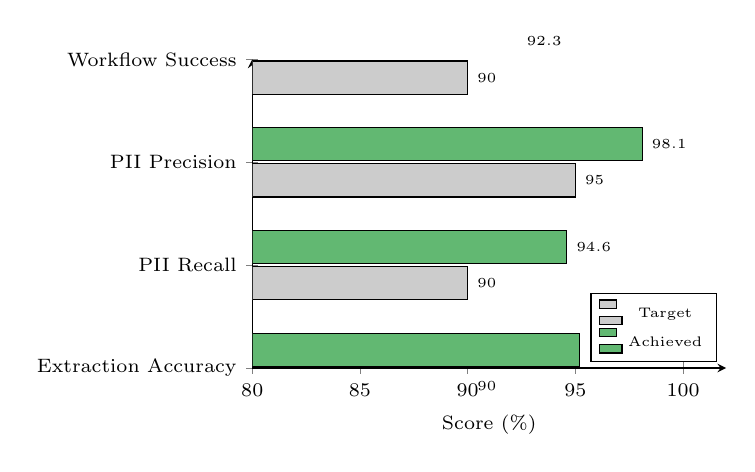
\begin{tikzpicture}
\begin{axis}[
  xbar,width=7.6cm,height=5.5cm,
  xlabel={Score (\%)},
  symbolic y coords={WorkflowSuccess,PIIPrecision,
    PIIRecall,ExtractionAccuracy},
  yticklabels={Workflow Success,PII Precision,
    PII Recall,Extraction Accuracy},
  ytick=data,
  xmin=80,xmax=102,
  nodes near coords,
  nodes near coords align={horizontal},
  nodes near coords style={font=\tiny\bfseries},
  bar width=0.42cm,
  axis x line=bottom,axis y line=left,
  tick label style={font=\scriptsize},
  xlabel style={font=\scriptsize},
  xtick={80,85,90,95,100},
  legend style={at={(0.98,0.02)},anchor=south east,font=\tiny},
]
\addplot[fill=black!20,bar shift=-0.23cm] coordinates {
  (90,ExtractionAccuracy)(95,PIIRecall)
  (90,PIIPrecision)(90,WorkflowSuccess)};
\addplot[fill=success!75,bar shift=0.23cm] coordinates {
  (92.3,ExtractionAccuracy)(98.1,PIIRecall)
  (94.6,PIIPrecision)(95.2,WorkflowSuccess)};
\legend{Target,Achieved}
\end{axis}
\end{tikzpicture}

\column{0.45\textwidth}
\vspace{4pt}
\textbf{Dataset:} 28 documents, 6 types, international coverage
(US, India, UK, Germany, Canada)

\vspace{6pt}
\begin{tabular}{@{}llll@{}}
\toprule
\rowcolor{primary!12}
\textbf{Metric} & \textbf{Target} & \textbf{Got} & \\
\midrule
\rowcolor{success!10}
Extraction  & 90\% & \textbf{92.3\%} &
  \textcolor{success}{\faCheckCircle} \\
\rowcolor{success!10}
PII Recall  & 95\% & \textbf{98.1\%} &
  \textcolor{success}{\faCheckCircle} \\
\rowcolor{success!10}
PII Precision & 90\% & \textbf{94.6\%} &
  \textcolor{success}{\faCheckCircle} \\
\rowcolor{success!10}
Workflow    & 90\% & \textbf{95.2\%} &
  \textcolor{success}{\faCheckCircle} \\
\rowcolor{success!10}
P95 Latency & $\leq$4 s & \textbf{1.8 s} &
  \textcolor{success}{\faCheckCircle} \\
\bottomrule
\end{tabular}

\vspace{8pt}
\begin{tcolorbox}[hibox=success]
\scriptsize
\textbf{All 5 targets met.}
Groq's 300+ tokens/sec drives sub-2 s
end-to-end latency across all 6 agents.
Medical PII recall \textbf{99.1\%} --- highest of all types.
\end{tcolorbox}
\end{columns}
\end{frame}

%==========================================================
\section{Salient Features}
%==========================================================

\begin{frame}{Salient Features}
\begin{columns}[T]
\column{0.48\textwidth}

\begin{tcolorbox}[titled,title={\faProjectDiagram~Agentic LangGraph Pipeline}]
\scriptsize
Stateful graph --- \texttt{DocumentState} shared across all nodes.
Conditional routing: self-repair fires \textit{only} when needed.
\textbf{MemorySaver} checkpoints after every node; crash-resilient.
\end{tcolorbox}

\vspace{5pt}
\begin{tcolorbox}[titled,title={\faShieldAlt~International PII Coverage}]
\scriptsize
Presidio baseline + \textbf{custom Indian regex recognisers}:
Aadhaar, PAN, GSTIN, Passport, Voter ID, UPI, IFSC.
LLM fills gaps Presidio misses. Merge-deduplication prevents
double-masking.
\end{tcolorbox}

\vspace{5pt}
\begin{tcolorbox}[titled,title={\faWrench~Self-Healing Extraction}]
\scriptsize
60+ field aliases + two-mode self-repair fills gaps
without overwriting valid data.
4-strategy JSON parser handles truncated / malformed LLM output.
\end{tcolorbox}

\column{0.48\textwidth}

\begin{tcolorbox}[titled,title={\faBolt~4-Tier Zero-Downtime LLM Chain}]
\scriptsize
Groq \textrightarrow{} Bedrock \textrightarrow{} HuggingFace
\textrightarrow{} Local phi-2.
Tenacity retries with exponential backoff (2 s / 4 s / 8 s).
No single provider failure can stop the pipeline.
\end{tcolorbox}

\vspace{5pt}
\begin{tcolorbox}[titled,title={\faBalanceScale~Responsible AI Logging}]
\scriptsize
Every agent decision logged: \texttt{agent\_name},
\texttt{llm\_provider}, \texttt{latency\_ms}, \texttt{status},
input/output summary.
Exported as \textbf{structured CSV} --- GDPR Art.~22 ready.
\end{tcolorbox}

\vspace{5pt}
\begin{tcolorbox}[titled,title={\faFileAlt~Universal Document Ingestion}]
\scriptsize
PDF (digital + scanned), DOCX, TXT, PPTX, XLSX, PNG, JPG, TIFF.
Tesseract OCR fallback for image-only files.
Auto-detects mixed digital+scanned PDFs.
\end{tcolorbox}

\end{columns}
\end{frame}

%==========================================================
\section{Demo}
%==========================================================

\begin{frame}{Demo}
\begin{columns}[T]
\column{0.50\textwidth}
\begin{tcolorbox}[titled,title={\faDesktop~Streamlit UI --- \texttt{:8501}}]
\begin{enumerate}\small\setlength\itemsep{4pt}
  \item \textbf{Upload} any PDF / DOCX / TXT / image,
        or select from \textbf{34 pre-loaded sample docs}
  \item Results in tabbed view:
    \begin{itemize}\scriptsize
      \item Classification (type, confidence, reasoning)
      \item Extraction (full JSON fields)
      \item Validation (status, warnings)
      \item Redaction (original vs.\ masked, side-by-side)
      \item Metrics (accuracy, PII scores)
      \item Responsible AI (trace log table)
    \end{itemize}
  \item \textbf{Download} JSON report + CSV audit log
\end{enumerate}
\end{tcolorbox}

\column{0.46\textwidth}
\begin{tcolorbox}[titled,title={\faServer~FastAPI --- \texttt{:8000/docs}}]
\begin{tabular}{@{}ll@{}}
\texttt{GET /health} & LLM availability \\
\texttt{POST /process} & process by path \\
\texttt{POST /upload} & multipart upload \\
\end{tabular}
\end{tcolorbox}

\vspace{8pt}
\begin{tcolorbox}[hibox=accent,
  title={\faPlayCircle~Demo Steps},
  fonttitle=\bfseries\small,coltitle=white,
  attach boxed title to top left,
  boxed title style={colback=accent,sharp corners}]
\scriptsize
\textbf{1.} \texttt{streamlit run streamlit\_app.py}\\[3pt]
\textbf{2.} Upload \texttt{sample\_medical\_record.txt}\\[3pt]
\textbf{3.} Walk through all 6 tabs\\[3pt]
\textbf{4.} Show side-by-side PII redaction\\[3pt]
\textbf{5.} Download JSON report
\end{tcolorbox}
\end{columns}
\end{frame}

%==========================================================
\section{Future Scope}
%==========================================================

\begin{frame}{Future Scope}
\begin{columns}[T]
\column{0.48\textwidth}
\begin{tcolorbox}[titled,title={\faMapSigns~Near-Term (3--6 months)}]
\begin{itemize}\small\setlength\itemsep{5pt}
  \item \textbf{Batch processing} --- async Celery queue
        for processing hundreds of docs via \texttt{/batch}
        endpoint
  \item \textbf{Table extraction} --- Camelot / pdfplumber
        for complex financial statements (multi-page PDFs)
  \item \textbf{FAISS semantic lookup} --- retrieve similar
        past docs to augment extraction context
        (scaffolding already in \texttt{utils/faiss\_manager.py})
  \item \textbf{Multi-language OCR} --- Tesseract multi-lang
        packs for Hindi, Arabic, Chinese documents
\end{itemize}
\end{tcolorbox}

\column{0.48\textwidth}
\begin{tcolorbox}[titled,title={\faRocket~Long-Term (6--12 months)}]
\begin{itemize}\small\setlength\itemsep{5pt}
  \item \textbf{Fine-tuned classifier} ---
        DistilBERT trained on domain-specific docs;
        replaces LLM for classification (faster, cheaper)
  \item \textbf{Active learning loop} --- human corrections
        feed back into training to improve extraction
        accuracy over time
  \item \textbf{Cloud deployment} ---
        Docker + AWS ECS / Lambda with S3 document storage
  \item \textbf{Differential privacy} --- calibrated noise
        on aggregate metrics to protect sensitive statistics
\end{itemize}
\end{tcolorbox}
\end{columns}
\end{frame}

%------ THANK YOU ------
\begin{frame}[plain]
\begin{tikzpicture}[remember picture,overlay]
  \fill[primary](current page.north west)
    rectangle([yshift=-1.8cm]current page.north east);
  \fill[accent]([yshift=-1.8cm]current page.north west)
    rectangle([yshift=-1.95cm]current page.north east);
  \fill[primary!80](current page.south west)
    rectangle([yshift=1.1cm]current page.south east);
\end{tikzpicture}

\vspace{0.4cm}
\begin{center}
  {\color{white}\fontsize{28}{33}\selectfont\bfseries Thank You!}\\[6pt]
  {\color{white!80}\large Questions \& Live Demo}\\[10pt]
  {\color{accent}\rule{8cm}{1.4pt}}\\[10pt]
  \begin{tikzpicture}
    \node[fill=white,rounded corners=7pt,inner sep=10pt,
          draw=primary!40,line width=1pt]{%
      \begin{tabular}{c}
        \color{primary}\textbf{Agentic Document Processor}\\[5pt]
        \scriptsize\color{darkgray!80}
        \faGithub~~\texttt{github.com/Charan-L574/agentic-doc-processor}\\[4pt]
        \faDesktop~~Streamlit UI:\quad\texttt{localhost:8501}\\[4pt]
        \faServer~~FastAPI Swagger:\quad\texttt{localhost:8000/docs}\\
      \end{tabular}};
  \end{tikzpicture}
  \vspace{8pt}

  \begin{tcolorbox}[enhanced,width=8cm,colback=accent!10,colframe=accent,
    sharp corners,boxrule=1pt,halign=center]
    \small\textbf{Start:}\quad
    \ttfamily\footnotesize
    \textcolor{primary}{streamlit run} streamlit\_app.py\\[-1pt]
    \textcolor{primary}{uvicorn} api.main:app --reload
  \end{tcolorbox}
\end{center}
\end{frame}

\end{document}
